% Options for packages loaded elsewhere
\PassOptionsToPackage{unicode}{hyperref}
\PassOptionsToPackage{hyphens}{url}
%
\documentclass[
]{article}
\usepackage{amsmath,amssymb}
\usepackage{lmodern}
\usepackage{iftex}
\ifPDFTeX
  \usepackage[T1]{fontenc}
  \usepackage[utf8]{inputenc}
  \usepackage{textcomp} % provide euro and other symbols
\else % if luatex or xetex
  \usepackage{unicode-math}
  \defaultfontfeatures{Scale=MatchLowercase}
  \defaultfontfeatures[\rmfamily]{Ligatures=TeX,Scale=1}
\fi
% Use upquote if available, for straight quotes in verbatim environments
\IfFileExists{upquote.sty}{\usepackage{upquote}}{}
\IfFileExists{microtype.sty}{% use microtype if available
  \usepackage[]{microtype}
  \UseMicrotypeSet[protrusion]{basicmath} % disable protrusion for tt fonts
}{}
\makeatletter
\@ifundefined{KOMAClassName}{% if non-KOMA class
  \IfFileExists{parskip.sty}{%
    \usepackage{parskip}
  }{% else
    \setlength{\parindent}{0pt}
    \setlength{\parskip}{6pt plus 2pt minus 1pt}}
}{% if KOMA class
  \KOMAoptions{parskip=half}}
\makeatother
\usepackage{xcolor}
\usepackage[margin=1in]{geometry}
\usepackage{color}
\usepackage{fancyvrb}
\newcommand{\VerbBar}{|}
\newcommand{\VERB}{\Verb[commandchars=\\\{\}]}
\DefineVerbatimEnvironment{Highlighting}{Verbatim}{commandchars=\\\{\}}
% Add ',fontsize=\small' for more characters per line
\usepackage{framed}
\definecolor{shadecolor}{RGB}{248,248,248}
\newenvironment{Shaded}{\begin{snugshade}}{\end{snugshade}}
\newcommand{\AlertTok}[1]{\textcolor[rgb]{0.94,0.16,0.16}{#1}}
\newcommand{\AnnotationTok}[1]{\textcolor[rgb]{0.56,0.35,0.01}{\textbf{\textit{#1}}}}
\newcommand{\AttributeTok}[1]{\textcolor[rgb]{0.77,0.63,0.00}{#1}}
\newcommand{\BaseNTok}[1]{\textcolor[rgb]{0.00,0.00,0.81}{#1}}
\newcommand{\BuiltInTok}[1]{#1}
\newcommand{\CharTok}[1]{\textcolor[rgb]{0.31,0.60,0.02}{#1}}
\newcommand{\CommentTok}[1]{\textcolor[rgb]{0.56,0.35,0.01}{\textit{#1}}}
\newcommand{\CommentVarTok}[1]{\textcolor[rgb]{0.56,0.35,0.01}{\textbf{\textit{#1}}}}
\newcommand{\ConstantTok}[1]{\textcolor[rgb]{0.00,0.00,0.00}{#1}}
\newcommand{\ControlFlowTok}[1]{\textcolor[rgb]{0.13,0.29,0.53}{\textbf{#1}}}
\newcommand{\DataTypeTok}[1]{\textcolor[rgb]{0.13,0.29,0.53}{#1}}
\newcommand{\DecValTok}[1]{\textcolor[rgb]{0.00,0.00,0.81}{#1}}
\newcommand{\DocumentationTok}[1]{\textcolor[rgb]{0.56,0.35,0.01}{\textbf{\textit{#1}}}}
\newcommand{\ErrorTok}[1]{\textcolor[rgb]{0.64,0.00,0.00}{\textbf{#1}}}
\newcommand{\ExtensionTok}[1]{#1}
\newcommand{\FloatTok}[1]{\textcolor[rgb]{0.00,0.00,0.81}{#1}}
\newcommand{\FunctionTok}[1]{\textcolor[rgb]{0.00,0.00,0.00}{#1}}
\newcommand{\ImportTok}[1]{#1}
\newcommand{\InformationTok}[1]{\textcolor[rgb]{0.56,0.35,0.01}{\textbf{\textit{#1}}}}
\newcommand{\KeywordTok}[1]{\textcolor[rgb]{0.13,0.29,0.53}{\textbf{#1}}}
\newcommand{\NormalTok}[1]{#1}
\newcommand{\OperatorTok}[1]{\textcolor[rgb]{0.81,0.36,0.00}{\textbf{#1}}}
\newcommand{\OtherTok}[1]{\textcolor[rgb]{0.56,0.35,0.01}{#1}}
\newcommand{\PreprocessorTok}[1]{\textcolor[rgb]{0.56,0.35,0.01}{\textit{#1}}}
\newcommand{\RegionMarkerTok}[1]{#1}
\newcommand{\SpecialCharTok}[1]{\textcolor[rgb]{0.00,0.00,0.00}{#1}}
\newcommand{\SpecialStringTok}[1]{\textcolor[rgb]{0.31,0.60,0.02}{#1}}
\newcommand{\StringTok}[1]{\textcolor[rgb]{0.31,0.60,0.02}{#1}}
\newcommand{\VariableTok}[1]{\textcolor[rgb]{0.00,0.00,0.00}{#1}}
\newcommand{\VerbatimStringTok}[1]{\textcolor[rgb]{0.31,0.60,0.02}{#1}}
\newcommand{\WarningTok}[1]{\textcolor[rgb]{0.56,0.35,0.01}{\textbf{\textit{#1}}}}
\usepackage{graphicx}
\makeatletter
\def\maxwidth{\ifdim\Gin@nat@width>\linewidth\linewidth\else\Gin@nat@width\fi}
\def\maxheight{\ifdim\Gin@nat@height>\textheight\textheight\else\Gin@nat@height\fi}
\makeatother
% Scale images if necessary, so that they will not overflow the page
% margins by default, and it is still possible to overwrite the defaults
% using explicit options in \includegraphics[width, height, ...]{}
\setkeys{Gin}{width=\maxwidth,height=\maxheight,keepaspectratio}
% Set default figure placement to htbp
\makeatletter
\def\fps@figure{htbp}
\makeatother
\setlength{\emergencystretch}{3em} % prevent overfull lines
\providecommand{\tightlist}{%
  \setlength{\itemsep}{0pt}\setlength{\parskip}{0pt}}
\setcounter{secnumdepth}{-\maxdimen} % remove section numbering
\ifLuaTeX
  \usepackage{selnolig}  % disable illegal ligatures
\fi
\IfFileExists{bookmark.sty}{\usepackage{bookmark}}{\usepackage{hyperref}}
\IfFileExists{xurl.sty}{\usepackage{xurl}}{} % add URL line breaks if available
\urlstyle{same} % disable monospaced font for URLs
\hypersetup{
  pdftitle={Real data: CAPE Negative},
  pdfauthor={Itziar Irigoien, Patricia Mas-Bermejo, Sergi Papiol, Neus Barrantes-Vidal,; Araceli Rosa, and Concepción Arenas},
  hidelinks,
  pdfcreator={LaTeX via pandoc}}

\title{Real data: CAPE Negative}
\usepackage{etoolbox}
\makeatletter
\providecommand{\subtitle}[1]{% add subtitle to \maketitle
  \apptocmd{\@title}{\par {\large #1 \par}}{}{}
}
\makeatother
\subtitle{In: A guide to test association between Polygenic Risk Scores
and psychological and psychiatric traits: practical examples}
\author{Itziar Irigoien, Patricia Mas-Bermejo, Sergi Papiol, Neus
Barrantes-Vidal, \and Araceli Rosa, and Concepción Arenas}
\date{}

\begin{document}
\maketitle

\hypertarget{working-flow-and-code}{%
\subsection{Working flow and code}\label{working-flow-and-code}}

In this real data set there are 106 PRS, and a \textbf{continuous Trait}
(\(CAPE_{Negative}\)), with sex, age, and two Principal Components as
covariates. For more details see Section 7 in the paper.

\begin{itemize}
\tightlist
\item
  Data reading
\end{itemize}

\begin{Shaded}
\begin{Highlighting}[]
\NormalTok{dat }\OtherTok{\textless{}{-}} \FunctionTok{read.table}\NormalTok{(}\StringTok{"Real\_data\_Negative.csv"}\NormalTok{, }\AttributeTok{header=}\ConstantTok{TRUE}\NormalTok{, }\AttributeTok{sep=}\StringTok{"}\SpecialCharTok{\textbackslash{}t}\StringTok{"}\NormalTok{, }\AttributeTok{dec=}\StringTok{"."}\NormalTok{)}
\FunctionTok{names}\NormalTok{(dat) }\CommentTok{\#}
\end{Highlighting}
\end{Shaded}

\begin{verbatim}
##   [1] "ID"            "Sex"           "Age"           "CAPE_Negative"
##   [5] "PRS.1"         "PRS.2"         "PRS.3"         "PRS.4"        
##   [9] "PRS.5"         "PRS.6"         "PRS.7"         "PRS.8"        
##  [13] "PRS.9"         "PRS.10"        "PRS.11"        "PRS.12"       
##  [17] "PRS.13"        "PRS.14"        "PRS.15"        "PRS.16"       
##  [21] "PRS.17"        "PRS.18"        "PRS.19"        "PRS.20"       
##  [25] "PRS.21"        "PRS.22"        "PRS.23"        "PRS.24"       
##  [29] "PRS.25"        "PRS.26"        "PRS.27"        "PRS.28"       
##  [33] "PRS.29"        "PRS.30"        "PRS.31"        "PRS.32"       
##  [37] "PRS.33"        "PRS.34"        "PRS.35"        "PRS.36"       
##  [41] "PRS.37"        "PRS.38"        "PRS.39"        "PRS.40"       
##  [45] "PRS.41"        "PRS.42"        "PRS.43"        "PRS.44"       
##  [49] "PRS.45"        "PRS.46"        "PRS.47"        "PRS.48"       
##  [53] "PRS.49"        "PRS.50"        "PRS.51"        "PRS.52"       
##  [57] "PRS.53"        "PRS.54"        "PRS.55"        "PRS.56"       
##  [61] "PRS.57"        "PRS.58"        "PRS.59"        "PRS.60"       
##  [65] "PRS.61"        "PRS.62"        "PRS.63"        "PRS.64"       
##  [69] "PRS.65"        "PRS.66"        "PRS.67"        "PRS.68"       
##  [73] "PRS.69"        "PRS.70"        "PRS.71"        "PRS.72"       
##  [77] "PRS.73"        "PRS.74"        "PRS.75"        "PRS.76"       
##  [81] "PRS.77"        "PRS.78"        "PRS.79"        "PRS.80"       
##  [85] "PRS.81"        "PRS.82"        "PRS.83"        "PRS.84"       
##  [89] "PRS.85"        "PRS.86"        "PRS.87"        "PRS.88"       
##  [93] "PRS.89"        "PRS.90"        "PRS.91"        "PRS.92"       
##  [97] "PRS.93"        "PRS.94"        "PRS.95"        "PRS.96"       
## [101] "PRS.97"        "PRS.98"        "PRS.99"        "PRS.100"      
## [105] "PRS.101"       "PRS.102"       "PRS.103"       "PRS.104"      
## [109] "PRS.105"       "PRS.106"       "PC1"           "PC2"
\end{verbatim}

\begin{Shaded}
\begin{Highlighting}[]
\NormalTok{dat }\OtherTok{\textless{}{-}}\NormalTok{ dat[, }\SpecialCharTok{{-}}\DecValTok{1}\NormalTok{]}
\end{Highlighting}
\end{Shaded}

Important! Check that all variables you are interested in are properly
read and that there are not other variables you do not need.

\bigskip

\begin{itemize}
\tightlist
\item
  Do not forget to declare the categorical variables as factors.
\end{itemize}

\begin{Shaded}
\begin{Highlighting}[]
\NormalTok{dat}\SpecialCharTok{$}\NormalTok{Sex }\OtherTok{\textless{}{-}} \FunctionTok{as.factor}\NormalTok{(dat}\SpecialCharTok{$}\NormalTok{Sex)}
\end{Highlighting}
\end{Shaded}

\hypertarget{what-full-model-should-be-considered}{%
\subsection{1. What full model should be
considered?}\label{what-full-model-should-be-considered}}

First, given a particular PRS (named PRS.i), consider all the possible
full models:

\begin{itemize}
\tightlist
\item
  FM\(_{WI}\) : Trait versus PRS.i + Sex + Age + PC1 + PC2
\item
  FM\(_{Sex}\): Trait versus PRS.i + Sex + PRS.i · Sex + Age + PC1 + PC2
\end{itemize}

\hypertarget{how-to-make-a-prs-ranking-to-find-the-important-ones}{%
\subsection{2. How to make a PRS ranking to find the important
ones?}\label{how-to-make-a-prs-ranking-to-find-the-important-ones}}

As is described in the paper, for each model, calculate the coefficient
of determination \(R^2\) and calculate the sum:
\(S = R^2_{WI} + R^2_{Sex}\).

According to S, list the PRSs in decreasing order:

\begin{Shaded}
\begin{Highlighting}[]
\NormalTok{out }\OtherTok{\textless{}{-}} \FunctionTok{orderR2}\NormalTok{(dat, }\AttributeTok{yname=}\StringTok{"CAPE\_Negative"}\NormalTok{, }\AttributeTok{prsname =} \StringTok{"PRS."}\NormalTok{)}
\FunctionTok{head}\NormalTok{(out)}
\end{Highlighting}
\end{Shaded}

\begin{verbatim}
##            Model1     Model2        Sum
## PRS.13 0.04743339 0.04930427 0.09673766
## PRS.12 0.04450825 0.04791485 0.09242311
## PRS.14 0.04102906 0.04398352 0.08501259
## PRS.70 0.03997513 0.04044623 0.08042136
## PRS.65 0.03986674 0.04044801 0.08031474
## PRS.69 0.03990297 0.04039181 0.08029478
\end{verbatim}

\begin{Shaded}
\begin{Highlighting}[]
\NormalTok{mainfilename }\OtherTok{\textless{}{-}} \StringTok{"Real\_example\_CAPE\_Negative"}
\NormalTok{filename }\OtherTok{\textless{}{-}} \FunctionTok{paste0}\NormalTok{(mainfilename, }\StringTok{"\_Ordered\_PRS.csv"}\NormalTok{)}
\FunctionTok{write.csv2}\NormalTok{(out,}\AttributeTok{file=}\NormalTok{filename)}
\end{Highlighting}
\end{Shaded}

Plot the sum of coefficients of determination \(S_{R^2}\). Lines: in
blue the median; in black the mean.

\begin{Shaded}
\begin{Highlighting}[]
\NormalTok{out }\OtherTok{\textless{}{-}} \FunctionTok{data.frame}\NormalTok{(out) }
\NormalTok{nPRS }\OtherTok{\textless{}{-}} \FunctionTok{dim}\NormalTok{(out)[}\DecValTok{1}\NormalTok{]}
\NormalTok{select }\OtherTok{\textless{}{-}} \FunctionTok{grep}\NormalTok{(}\StringTok{"Model"}\NormalTok{, }\FunctionTok{names}\NormalTok{(out), }\AttributeTok{value=}\ConstantTok{FALSE}\NormalTok{)}
\NormalTok{out}\SpecialCharTok{$}\NormalTok{effect }\OtherTok{\textless{}{-}}\NormalTok{ out}\SpecialCharTok{$}\NormalTok{Sum}
\NormalTok{sds }\OtherTok{\textless{}{-}} \FunctionTok{apply}\NormalTok{(out[, select], }\DecValTok{1}\NormalTok{, sd)}
\NormalTok{out}\SpecialCharTok{$}\NormalTok{lower }\OtherTok{\textless{}{-}}\NormalTok{ out}\SpecialCharTok{$}\NormalTok{effect }\SpecialCharTok{{-}}\NormalTok{ sds}
\NormalTok{out}\SpecialCharTok{$}\NormalTok{upper }\OtherTok{\textless{}{-}}\NormalTok{ out}\SpecialCharTok{$}\NormalTok{effect }\SpecialCharTok{+}\NormalTok{ sds}
\NormalTok{out}\SpecialCharTok{$}\NormalTok{rank }\OtherTok{\textless{}{-}}\NormalTok{ nPRS}\SpecialCharTok{:}\DecValTok{1}

\NormalTok{n }\OtherTok{\textless{}{-}} \FunctionTok{dim}\NormalTok{(out)[}\DecValTok{1}\NormalTok{]}
\FunctionTok{ggplot}\NormalTok{(}\AttributeTok{data=}\NormalTok{out, }\FunctionTok{aes}\NormalTok{(}\AttributeTok{y=}\NormalTok{rank, }\AttributeTok{x=}\NormalTok{effect, }\AttributeTok{xmin=}\NormalTok{lower, }\AttributeTok{xmax=}\NormalTok{upper)) }\SpecialCharTok{+}
  \FunctionTok{geom\_point}\NormalTok{() }\SpecialCharTok{+}
  \FunctionTok{geom\_errorbarh}\NormalTok{(}\AttributeTok{height=}\NormalTok{.}\DecValTok{1}\NormalTok{) }\SpecialCharTok{+}
  \FunctionTok{scale\_y\_continuous}\NormalTok{(}\AttributeTok{name=}\ConstantTok{NULL}\NormalTok{, }\AttributeTok{breaks=}\NormalTok{ n}\SpecialCharTok{:}\DecValTok{1}\NormalTok{, }\AttributeTok{labels=}\FunctionTok{row.names}\NormalTok{(out), }\AttributeTok{position=}\StringTok{"right"}\NormalTok{) }\SpecialCharTok{+}
  \FunctionTok{labs}\NormalTok{(}\AttributeTok{title=}\StringTok{\textquotesingle{}\textquotesingle{}}\NormalTok{, }\AttributeTok{x=}\StringTok{\textquotesingle{}Sum R\^{}2\textquotesingle{}}\NormalTok{, }\AttributeTok{y =} \StringTok{\textquotesingle{}PRS\textquotesingle{}}\NormalTok{) }\SpecialCharTok{+}
  \FunctionTok{geom\_vline}\NormalTok{(}\AttributeTok{xintercept=}\FunctionTok{mean}\NormalTok{(out}\SpecialCharTok{$}\NormalTok{effect), }\AttributeTok{color=}\StringTok{\textquotesingle{}black\textquotesingle{}}\NormalTok{, }\AttributeTok{linetype=}\StringTok{\textquotesingle{}dashed\textquotesingle{}}\NormalTok{) }\SpecialCharTok{+}
  \FunctionTok{geom\_vline}\NormalTok{(}\AttributeTok{xintercept=}\FunctionTok{median}\NormalTok{(out}\SpecialCharTok{$}\NormalTok{effect), }\AttributeTok{color=}\StringTok{\textquotesingle{}blue\textquotesingle{}}\NormalTok{, }\AttributeTok{linetype=}\StringTok{\textquotesingle{}dashed\textquotesingle{}}\NormalTok{) }\SpecialCharTok{+}
  \FunctionTok{theme\_minimal}\NormalTok{()}
\end{Highlighting}
\end{Shaded}

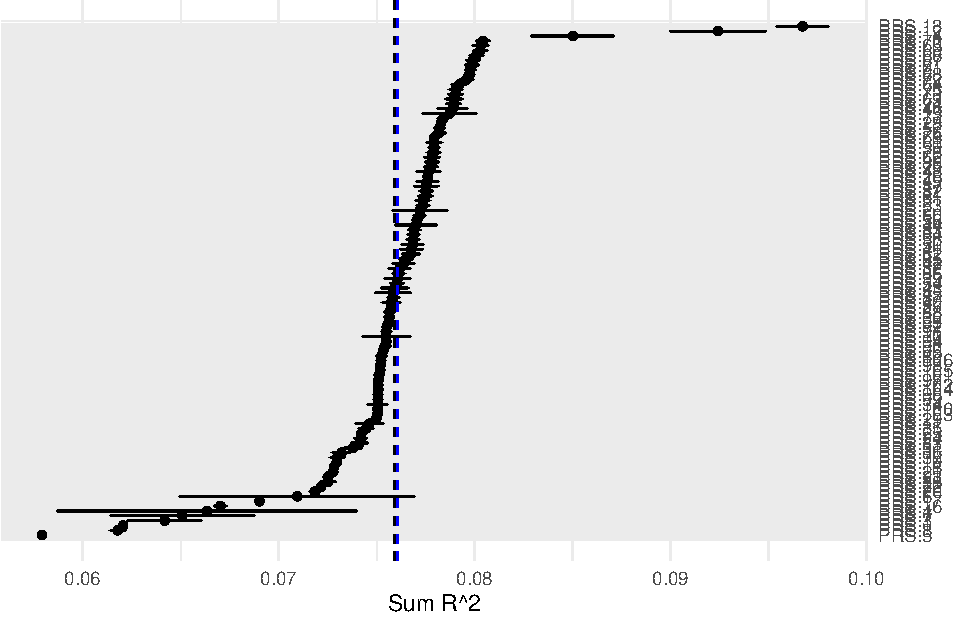
\includegraphics{Real_data_CAPE_Negative_code_files/figure-latex/unnamed-chunk-5-1.pdf}

According to the obtained results, first, PRS.13 is selected to analyse
its possible association with the \(CAPE_{Negative}\).

\hypertarget{which-model-of-all-the-possible-ones-should-be-used}{%
\subsection{3. Which model, of all the possible ones, should be
used?}\label{which-model-of-all-the-possible-ones-should-be-used}}

The following Figure represents the scatter plot of \(CAPE_{Negative}\)
versus PRS.13 separated by Sex group.

\begin{Shaded}
\begin{Highlighting}[]
\CommentTok{\# First candidate PRS.13}
\CommentTok{\# Plot it}
\FunctionTok{library}\NormalTok{(lattice) }
\FunctionTok{xyplot}\NormalTok{(CAPE\_Negative}\SpecialCharTok{\textasciitilde{}}\NormalTok{PRS}\FloatTok{.13}\SpecialCharTok{|}\NormalTok{Sex, }\AttributeTok{data=}\NormalTok{dat,  }\AttributeTok{type=}\FunctionTok{c}\NormalTok{(}\StringTok{"p"}\NormalTok{, }\StringTok{"r"}\NormalTok{))}
\end{Highlighting}
\end{Shaded}

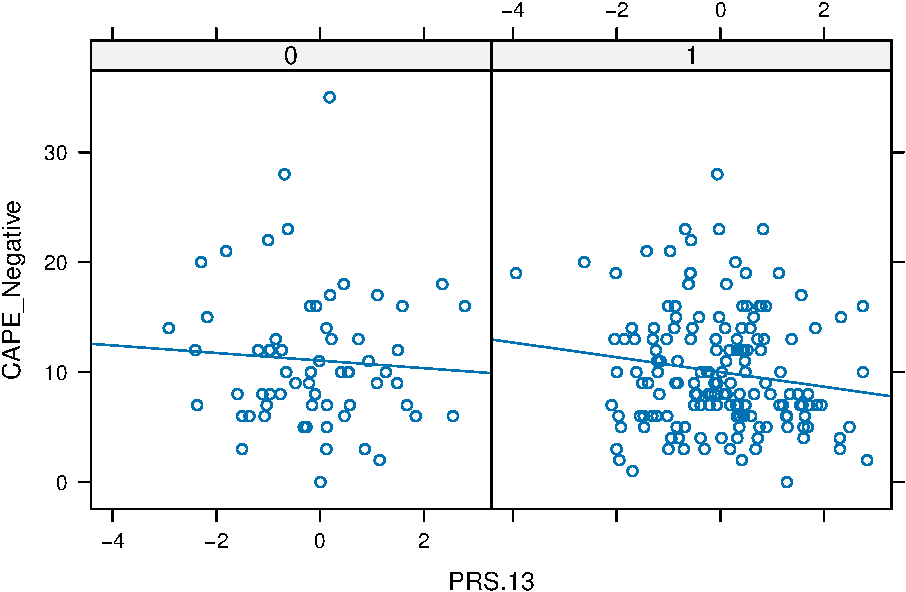
\includegraphics{Real_data_CAPE_Negative_code_files/figure-latex/unnamed-chunk-6-1.pdf}

The plots suggest that the interaction between the PRS.13 and the sex is
not relevant. Thus, we set the full model candidate (FM):
\(CAPE_{Negative} \sim PRS + Sex + Age + PC1 +PC2\).

\hypertarget{for-a-continuous-trait-what-steps-should-be-followed-for-a-correct-analysis}{%
\subsection{4. For a continuous trait, what steps should be followed for
a correct
analysis?}\label{for-a-continuous-trait-what-steps-should-be-followed-for-a-correct-analysis}}

\begin{itemize}
\tightlist
\item
  \textbf{4.1. How is the candidate model validated?}
\end{itemize}

First, we validate the normality of the errors and the constant variance
conditions (see the figures and the results of Shapiro test and Levene
test).

\begin{Shaded}
\begin{Highlighting}[]
\CommentTok{\#model}
\NormalTok{FM }\OtherTok{\textless{}{-}} \FunctionTok{lm}\NormalTok{(CAPE\_Negative }\SpecialCharTok{\textasciitilde{}}\NormalTok{ PRS}\FloatTok{.13} \SpecialCharTok{+}\NormalTok{ Sex }\SpecialCharTok{+}\NormalTok{ Age }\SpecialCharTok{+}\NormalTok{ PC1 }\SpecialCharTok{+}\NormalTok{ PC2, }\AttributeTok{data=}\NormalTok{dat)}
\CommentTok{\#qq{-}plot for normality }
\FunctionTok{plot}\NormalTok{(FM,}\DecValTok{2}\NormalTok{)   }
\end{Highlighting}
\end{Shaded}

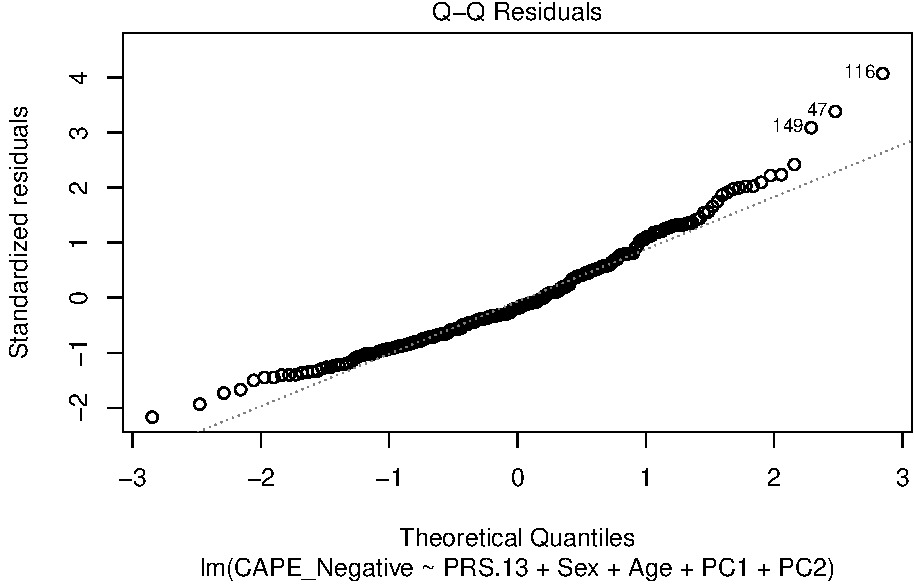
\includegraphics{Real_data_CAPE_Negative_code_files/figure-latex/unnamed-chunk-7-1.pdf}

The lack of normality of residuals is suggested by this last plot.

This supported by Shapiro's test:

\begin{Shaded}
\begin{Highlighting}[]
\CommentTok{\#Shapiro{-}Wilk test}
\FunctionTok{shapiro.test}\NormalTok{(FM}\SpecialCharTok{$}\NormalTok{residuals)}
\end{Highlighting}
\end{Shaded}

\begin{verbatim}
## 
##  Shapiro-Wilk normality test
## 
## data:  FM$residuals
## W = 0.95885, p-value = 4.335e-06
\end{verbatim}

\begin{Shaded}
\begin{Highlighting}[]
\CommentTok{\#plot for variances}
\NormalTok{d }\OtherTok{\textless{}{-}} \FunctionTok{fortify}\NormalTok{(FM)}
\FunctionTok{ggplot}\NormalTok{(d,}\FunctionTok{aes}\NormalTok{(}\AttributeTok{x=}\NormalTok{.fitted, }\AttributeTok{y=}\NormalTok{.stdresid, }\AttributeTok{colour=}\NormalTok{Sex)) }\SpecialCharTok{+}
  \FunctionTok{geom\_point}\NormalTok{() }\SpecialCharTok{+}
  \FunctionTok{geom\_hline}\NormalTok{(}\AttributeTok{yintercept=}\DecValTok{0}\NormalTok{, }\AttributeTok{col=}\StringTok{"red"}\NormalTok{)}\SpecialCharTok{+}
  \FunctionTok{facet\_wrap}\NormalTok{(.}\SpecialCharTok{\textasciitilde{}}\NormalTok{Sex)}
\end{Highlighting}
\end{Shaded}

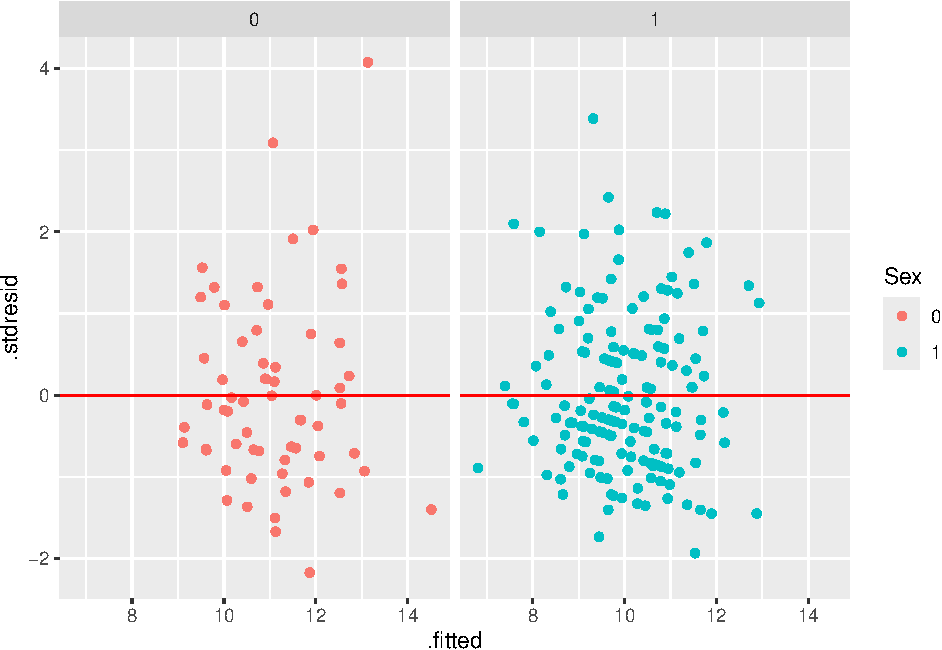
\includegraphics{Real_data_CAPE_Negative_code_files/figure-latex/unnamed-chunk-9-1.pdf}

\begin{Shaded}
\begin{Highlighting}[]
\CommentTok{\#Levene\textquotesingle{}s test}
\FunctionTok{leveneTest}\NormalTok{(.stdresid }\SpecialCharTok{\textasciitilde{}}\NormalTok{ Sex, }\AttributeTok{data=}\NormalTok{d)}
\end{Highlighting}
\end{Shaded}

\begin{verbatim}
## Levene's Test for Homogeneity of Variance (center = median)
##        Df F value Pr(>F)
## group   1  0.7613 0.3839
##       224
\end{verbatim}

All in all, it seems that there is lack of normality of residuals but
linearity and homocedasticity assumptions hold.

\begin{itemize}
\tightlist
\item
  \textbf{4.2. What can be done if any validation condition fails?}
\end{itemize}

We have two approaches to assess the possible association with PRS.13
and \(CAPE_{Negative}\): try a transformation or perform a permutation
test.

First we try the squared root transformation for the dependent variable:

\begin{Shaded}
\begin{Highlighting}[]
\NormalTok{dat}\SpecialCharTok{$}\NormalTok{TNegative }\OtherTok{\textless{}{-}} \FunctionTok{sqrt}\NormalTok{(dat}\SpecialCharTok{$}\NormalTok{CAPE\_Negative)}
\NormalTok{FM }\OtherTok{\textless{}{-}} \FunctionTok{lm}\NormalTok{(TNegative }\SpecialCharTok{\textasciitilde{}}\NormalTok{ PRS}\FloatTok{.13} \SpecialCharTok{+}\NormalTok{ Sex }\SpecialCharTok{+}\NormalTok{ Age }\SpecialCharTok{+}\NormalTok{ PC1 }\SpecialCharTok{+}\NormalTok{ PC2, }\AttributeTok{data=}\NormalTok{dat)}
\CommentTok{\#qq{-}plot for normality }
\FunctionTok{plot}\NormalTok{(FM,}\DecValTok{2}\NormalTok{)}
\end{Highlighting}
\end{Shaded}

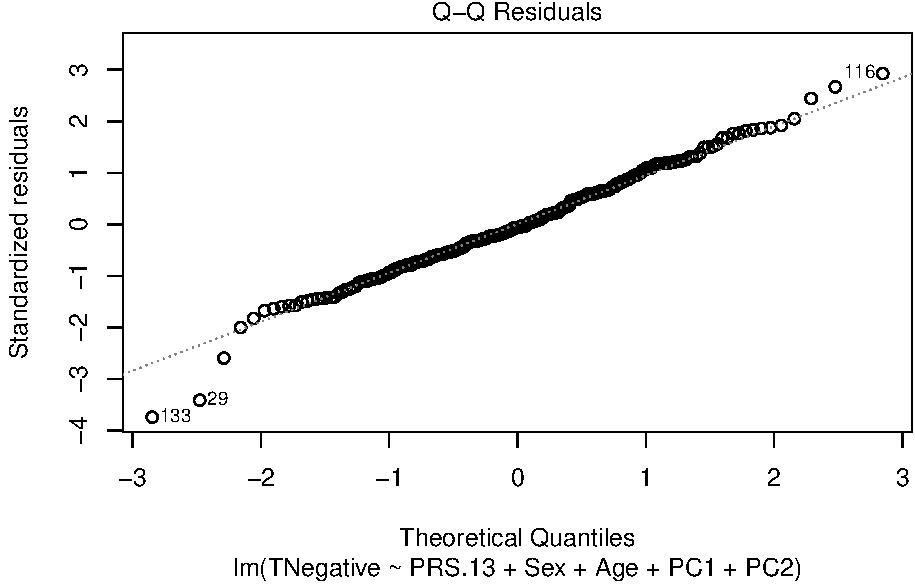
\includegraphics{Real_data_CAPE_Negative_code_files/figure-latex/unnamed-chunk-11-1.pdf}

\begin{Shaded}
\begin{Highlighting}[]
\CommentTok{\#Shapiro{-}Wilk test}
\FunctionTok{shapiro.test}\NormalTok{(FM}\SpecialCharTok{$}\NormalTok{residuals)}
\end{Highlighting}
\end{Shaded}

\begin{verbatim}
## 
##  Shapiro-Wilk normality test
## 
## data:  FM$residuals
## W = 0.98898, p-value = 0.08108
\end{verbatim}

It is suggested the transformation offered a solution for the lack of
normality. Furthermore,\ldots{}

\begin{Shaded}
\begin{Highlighting}[]
\CommentTok{\#plot for variances}
\NormalTok{d }\OtherTok{\textless{}{-}} \FunctionTok{fortify}\NormalTok{(FM)}
\FunctionTok{ggplot}\NormalTok{(d,}\FunctionTok{aes}\NormalTok{(}\AttributeTok{x=}\NormalTok{.fitted, }\AttributeTok{y=}\NormalTok{.stdresid, }\AttributeTok{colour=}\NormalTok{Sex)) }\SpecialCharTok{+}
  \FunctionTok{geom\_point}\NormalTok{() }\SpecialCharTok{+} 
  \FunctionTok{geom\_hline}\NormalTok{(}\AttributeTok{yintercept=}\DecValTok{0}\NormalTok{, }\AttributeTok{col=}\StringTok{"red"}\NormalTok{)}\SpecialCharTok{+}
  \FunctionTok{facet\_wrap}\NormalTok{(.}\SpecialCharTok{\textasciitilde{}}\NormalTok{Sex)}
\end{Highlighting}
\end{Shaded}

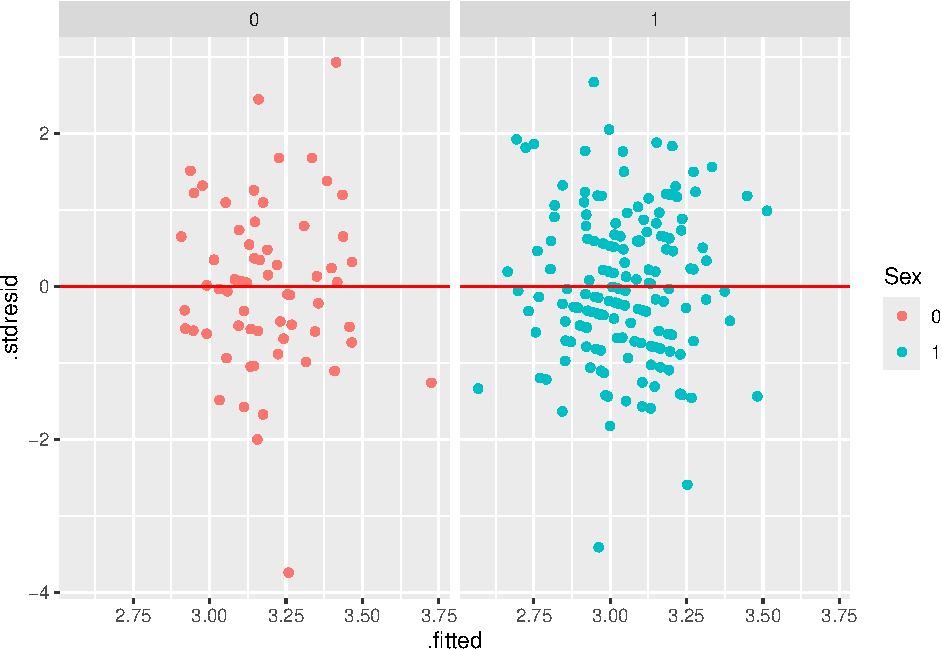
\includegraphics{Real_data_CAPE_Negative_code_files/figure-latex/unnamed-chunk-13-1.pdf}

\begin{Shaded}
\begin{Highlighting}[]
\CommentTok{\#Levene\textquotesingle{}s test}
\FunctionTok{leveneTest}\NormalTok{(.stdresid }\SpecialCharTok{\textasciitilde{}}\NormalTok{ Sex, }\AttributeTok{data=}\NormalTok{d)}
\end{Highlighting}
\end{Shaded}

\begin{verbatim}
## Levene's Test for Homogeneity of Variance (center = median)
##        Df F value Pr(>F)
## group   1  0.2998 0.5846
##       224
\end{verbatim}

\ldots results do not indicate evidence against homoscedasticity,
neither a pattern is observed that could indicate a lack of linearity.

Therefore, the model we build is given by:

\begin{Shaded}
\begin{Highlighting}[]
\FunctionTok{summary}\NormalTok{(FM)}
\end{Highlighting}
\end{Shaded}

\begin{verbatim}
## 
## Call:
## lm(formula = TNegative ~ PRS.13 + Sex + Age + PC1 + PC2, data = dat)
## 
## Residuals:
##     Min      1Q  Median      3Q     Max 
## -3.2590 -0.5534 -0.0529  0.5640  2.5020 
## 
## Coefficients:
##              Estimate Std. Error t value Pr(>|t|)    
## (Intercept)  3.013198   0.467855   6.440 7.39e-10 ***
## PRS.13      -0.101131   0.050141  -2.017   0.0449 *  
## Sex1        -0.142137   0.133729  -1.063   0.2890    
## Age          0.008634   0.021935   0.394   0.6943    
## PC1          3.796970   4.232105   0.897   0.3706    
## PC2          8.408721   4.206204   1.999   0.0468 *  
## ---
## Signif. codes:  0 '***' 0.001 '**' 0.01 '*' 0.05 '.' 0.1 ' ' 1
## 
## Residual standard error: 0.8837 on 220 degrees of freedom
##   (1 observation deleted due to missingness)
## Multiple R-squared:  0.04105,    Adjusted R-squared:  0.01926 
## F-statistic: 1.884 on 5 and 220 DF,  p-value: 0.09824
\end{verbatim}

The results show that PRS.13 is related with the \(\sqrt{Trait}\) in the
following way:

\[\widehat{\sqrt{Trait}} = 3.013 - 0.101\times PRS.13 - 0.142\times Sex + 0.009\times Age + 3.797\times PC1 + 8.409\times PC2,\]
where Sex takes values 0 or 1, depending on whether the individual under
study is male or female. See section 7.1 in the paper for more details.

On the other hand, based on the permutation approach:

\begin{Shaded}
\begin{Highlighting}[]
\NormalTok{NM }\OtherTok{\textless{}{-}} \FunctionTok{lm}\NormalTok{(CAPE\_Negative }\SpecialCharTok{\textasciitilde{}}\NormalTok{  Sex }\SpecialCharTok{+}\NormalTok{ Age }\SpecialCharTok{+}\NormalTok{ PC1 }\SpecialCharTok{+}\NormalTok{ PC2, }\AttributeTok{data=}\NormalTok{dat)}
\NormalTok{FM }\OtherTok{\textless{}{-}} \FunctionTok{lm}\NormalTok{(CAPE\_Negative }\SpecialCharTok{\textasciitilde{}}\NormalTok{ PRS}\FloatTok{.13} \SpecialCharTok{+}\NormalTok{ Sex }\SpecialCharTok{+}\NormalTok{ Age }\SpecialCharTok{+}\NormalTok{ PC1 }\SpecialCharTok{+}\NormalTok{ PC2, }\AttributeTok{data=}\NormalTok{dat)}
\NormalTok{outperm }\OtherTok{\textless{}{-}} \FunctionTok{dR2}\NormalTok{(}\AttributeTok{NullModel=}\NormalTok{NM, }\AttributeTok{FullModel=}\NormalTok{FM, }\AttributeTok{B=}\DecValTok{5000}\NormalTok{, }\AttributeTok{seed=}\DecValTok{165}\NormalTok{)}
\NormalTok{outperm}
\end{Highlighting}
\end{Shaded}

\begin{verbatim}
## $dR2
## [1] 0.01964777
## 
## $pvalue
## [1] 0.033
\end{verbatim}

We observe an increase of 0.0196 in the coefficient of determination
when the PRS.13 is included in the model and the permutation test
indicates it is significant.

\begin{itemize}
\tightlist
\item
  \textbf{Last step: We move to the next PRS.}
\end{itemize}

\end{document}
